%#-*- coding:utf-8 -*-
\documentclass[11pt,UTF8,hyperref,openany]{ctexbook}
\usepackage{amsmath}             %%%%多种的公式环境和数学命令
\usepackage{amssymb}             %%%%数学符号生成命令
\usepackage{array}               %%%%数组和表格
\usepackage{booktabs}            %%%%水平的表格线
\usepackage{calc}                %%%%四则运算
\usepackage{caption}             %%%%插图和表格
% \usepackage{ctex}                %%%%中文字体
\usepackage{ctexcap}             %%%%中文字体和标题
\usepackage{color}
\usepackage{fancyhdr}            %%%%页眉页脚设置
\usepackage{graphicx}            %%%%插图
\usepackage{geometry}            %%%%版面尺寸控制
\geometry{left=2cm, right=2cm, top=2cm, bottom=2cm, head=2cm, foot=1cm}
% head=?cm, headmap=?cm
\usepackage{hyperref}            %%%%超链接
\usepackage{ifthen}              %%%%条件
\usepackage{longtable}           %%%%跨页表格
\usepackage{lineno}              %%%%行号控制
\usepackage{listings}            %%%%C++
\usepackage{multicol}            %%%%多栏
\usepackage{makeidx}             %%%%索引
\usepackage{ntheorem}            %%%%定理设置
\usepackage{paralist}            %%%%列表
\usepackage{tabularx}            %%%%表格的列宽
\usepackage{titlesec}            %%%%章节标题
\usepackage{fancyvrb}            %%%%抄录
\usepackage{fontspec}            %%%%字体
\usepackage{titletoc}            %%%%目录格式
\usepackage{xcolor}              %%%%颜色处理
\usepackage{xeCJK}               %%%%中日朝文字处理
%%%%%%%%%%%%%%%%%%%%%%%%%%%%%%%%%%%%%%%%%%%%%%%%%%%%%%%%%% 
% C++
\definecolor{keywordcolor}{rgb}{0, 0, 1}
\lstset{breaklines}
\lstset{extendedchars=false}
\lstset{language=python, keywordstyle=\color{keywordcolor}\bfseries,
  basicstyle=\ttfamily,
  showstringspaces=false,
  captionpos=b
}

%%%%%%%%%%%%%%%%%%%%%%%%%%%%%%%%%%%%%%%%%%%%%%%%%%%%%%%%%% 
% newcommand
\newcommand{\mycmdA}{ }
\newcommand{\mycmdB}[1]{{\heiti #1}}
\newcommand{\mycmdC}[2]{$#1_1,#1_2,\dots,#1_#2$}


\author{xiaohai}
\title{matplotlib 学习笔记}

\begin{document}
% 页码的设置
\pagenumbering{Roman}

\maketitle

%%%%%%%%%%%%%%%%%%%%%%%%%%%%%%%%%%%%%%%%%%%%%%%%%%%%%%%%%% 
% 目录的设置
\titlecontents{chapter}[4em]{\addvspace{2.3mm}\bf}{%
  \contentslabel{4.0em}}{}{\titlerule*[5pt]{$\cdot$}\contentspage}
\titlecontents{section}[4em]{}{\contentslabel{2.5em}}{}{%
  \titlerule*[5pt]{$\cdot$}\contentspage}
\titlecontents{subsection}[7.2em]{}{\contentslabel{3.3em}}{}{%
  \titlerule*[5pt]{$\cdot$}\contentspage}
\tableofcontents

%%%%页码设置。

%%%%%%%%%%%%%%%%%%%%%%%%%%%%%%%%%%%%%%%%%%%%%%%%%%%%%%%%%% 
%#-*- coding:utf-8 -*-
\pagenumbering{arabic}
\chapter{TUTORIIALS}
\section{Introductory}
\subsection{Pyplot tutorial}
每一个Pyplot函数都会对图形做一些修改。例如,创建图形,在一个图形上创建画图面积,画线,装饰等。\\
plot()是一个通用的命令,其接受任意数量的参数。例如$plt.plot([1, 2, 3, 4], [1, 4, 9, 16])$,该函数也接受第三个参数,用来控
颜色和画图的格式。例如$plt.plot([1, 2, 3, 4], [1, 4, 9, 16], \textquoteleft ro \textquoteright)$
$plt.axis([0, 6, 0, 20])$用来指定图的范围。\newline
$plt.show()$展示图片。\newline
多图的控制plt.plot(t, t, \textquoteleft r--\textquoteright, t, $t^{2}$, \textquoteleft bs \textquoteright, t, $t^{3}$, \textquoteleft g\^{} \textquoteright)\newline
线也有很多的属性可以进行控制:\\
例如线宽linewidth $= 2.0$, dash style, antialiased等。\\
plt.plot(x, y, linewidth $= 2.0$)\\
可以使用setp()命令,一次进行多次的设定\\
\begin{verbatim}
lines = plt.plot(x1, y1, x2, y2)
#  use keyword args
plt.setp(lines, color='r', linewidth=2.0)
\end{verbatim}

\noindent{}Working with multiple figures and axes\\
pyplot has the concept of the current figure and the current axes.\\
gca()返回当前的axes,~ gcf()返回当前前figure\\
\begin{lstlisting}
import numpy as np
import matplotlib.pyplot as plt

def f(t):
    return np.exp(-t) * np.cos(2*np.pi*t)

t1 = np.arange(0.0, 5.0, 0.1)
t2 = np.arange(0.0, 5.0, 0.02)

plt.figure(1)
plt.subplot(211)
plt.plot(t1, f(t1), 'bo', t2, f(t2), 'k')

plt.subplot(212)
plt.plot(t2, np.cos(2*np.pi**t2), 'r--')
plt.show()
\end{lstlisting}
The figure() command 是个可选的参数,因为figure(1)是默认创建的.subplot()命令指定具体的行,列和fignum的范围从1到
numrows*numcols.其中subplot(211)等同于subpolt(2, 1, 1)这里也推荐使用后面的方式。\\
下面的方法设定图片的标题为"Easy as 1, 2, 3"\\
\hspace{1cm}plt.title("Easy as 1, 2, 3")\\

\subsection{Working with text}
命令text()可以在任何位置添加标题。而xlabel(), ylabel(), title()只能在指定的位置添加标题。

\begin{lstlisting}
import numpy as np
import matplotlib.pyplot as plt

np.random.seed(123)  

mu, sigma = 100, 15
x = mu + sigma * np.random.randn(10000)

n, bins, patches = plt.hist(x, 50, normed=1, facecolor='g', alpha=0.75)
plt.xlabel('Smarts')
plt.ylabel('Probability')
plt.title('Histogram of IQ')
plt.text(60, 0.25, r'$\mu=100,\ \sigma=15$')
plt.axis([40, 160, 0, 0.03])
plt.grid(True)
plt.show()
\end{lstlisting}
\begin{figure}
  \centering
  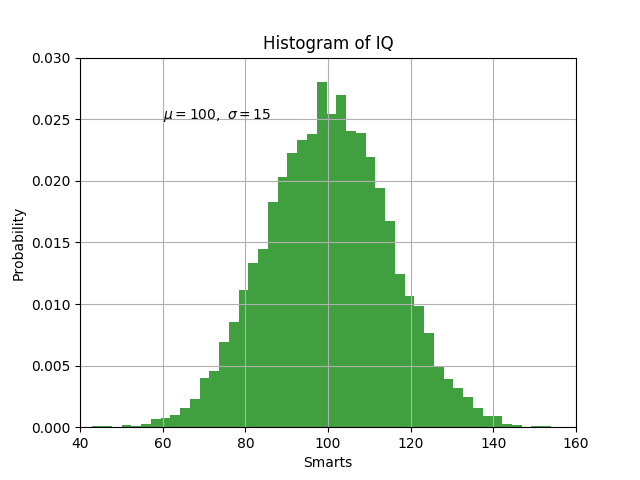
\includegraphics{./figure/text.png}
  \caption{text}
  \label{fig:text}
\end{figure}

All of the text() commands return an matplotlib.text.Text instance. you can customize the properties by passing keyword 
arguments into the text functions or using setp():\\
t = plt.xlabel("my data", fontsize=14, color="red")\\

matplotlib接受TeX的表达式在任何的text表达式中,
\begin{verbatim}
例如plt.title(r'$\Sigma_i=15$)
\end{verbatim}
其中r代表了一个raw字符串.
\subsection{注释text}
annotate()函数提供了一个简单的注释方法.\\
In the ananotation, there are two points to consider: the location being annotated represented by the argument xy and
the location of the text xytext.这两个参数都是(x, y)形式的tuples.\\
\begin{lstlisting}
import numpy as np
import matplotlib.pyplot as plt

ax = plt.subplot(1, 1, 1)
t = np.arange(0.0, 5.0, 0.01)
s = np.cos(2*np.pi*t)
line, = plt.plot(t, s, lw=2)

plt.annotate("local max", xy=(2, 1), xytext=(3, 1.5), arrowprops=dict(facecolor="black", shrink=0.05),)
plt.ylim(-2, 2)
plt.show()
\end{lstlisting}

\subsection{Logarithmic and other nonlinear axis}
非线性坐标轴的设定,例如logarithmic and logit scales,常用来处理跨度较大的范围.\\
例如
\begin{lstlisting}
plt.xscale("log")
plt.yscale("symlog", linthreshy=0.01)
plt.xscale("symlog")
plt.yscale("logit")
\end{lstlisting}

\subsection{Basic Example of using subplot2grid}
To use subplot2grid, you provide geometry of the grid and the location of the subplot in the grid. For a simple
single-cell subplot:\\
\begin{verbatim}
ax = plt.subplot3grid((2, 2), (0, 0))
is identical to
ax = plt.subplot(2, 2, 1)\\
To create a subplot that spans multiple cells(创建一个subplot横跨多个单元)
ax2 = plt.subplot2grid((3, 3), (1, 0), colspan=2)
ax3 = plt.subplot2grid((3, 3), (1, 0), rowspan=2)
\end{verbatim}

\subsection{GridSpec and SubplotSpec}
You can create GridSpec explicitly and use them to create a Subplot.\\
For example,
\begin{lstlisting}
ax = plt.subplot2grid((2, 2), (0, 0))
is equal to
import matplotlib.gridspec as gridspec
gs = gridspec.GridSpec(2, 2)
ax = plt.subplot(gs[0, 0])
\end{lstlisting}


\subsection{Legend guide}
\textbf{legend entry} A legend is made up of one or more legend entries.\\
\textbf{legend key} The colored marker to the left of each legend label.\\
\textbf{legend label} The text which describes the handle represented by the key.\\
为了完全的控制图例,一般会直接的在legend()中选择合适的handles.\\
\begin{lstlisting}
line_up, = plt.plot([1, 2, 3], label="Line 2")
line_down, = plt.plot([3, 2, 1], label="Line 1")
plt.legend(handles=[line_up, line_down])
\end{lstlisting}

\noindent{}在某些情况下,不可能去设定label of the handle, 因此我们可以传进去一个label的list.\\
\begin{lstlisting}
line_up, = plt.plot([1, 2, 3], label="Line 2")
line_down, = plt.plot([3, 2, 1], label="Line 1")
plt.legend([line_up, line_down], ["Line Up", "Line Down"])
\end{lstlisting}

\noindent{}手动创建legend
并不是所有的handles都可以被自动的传到automatically.因此我们需要手动的创建一个.\\
例如下面我们创建的一个红色的red color.\\
\begin{lstlisting}
import matplotlib.patches as mpatches
import matplotlib.pyplot as plt

red_patch = mpathces.Patch(color="red", label="The red data")
plt.legend(handles=[red_patch])

plt.show()
\end{lstlisting}




%%% Local Variables:
%%% mode: latex
%%% TeX-master: t
%%% End:


%%%%%%%%%%%%%%%%%%%%%%%%%%%%%%%%%%%%%%%%%%%%%%%%%%%%%%%%%% 
% \pagenumbering{arabic}
% % footnote
% \renewcommand{\thefootnote}{}
% \footnote{\heiti{ 作者简介}: 金小海,男}
% \footnote{\heiti{ 现在单位}: Sinap}
% % 将脚注的引用记数设为0.
% \setcounter{footnote}{0}
% \renewcommand{\thefootnote}{\arabic{footnote}}


%%%%%%%%%%%%%%%%%%%%%%%%%%%%%%%%%%%%%%%%%%%%%%%%%%%%%%%%%% 
% 附录
\appendix
\chapter{C++程序}
\section{Ising model}
\section{Monter carlo method}

%%%%%%%%%%%%%%%%%%%%%%%%%%%%%%%%%%%%%%%%%%%%%%%%%%%%%%%%%% 
% 参考文献
\begin{thebibliography}{99}
\bibitem[文献序号1]{检索名1}文献的信息1
\bibitem[文献序号2]{检索名2}文献的信息2
\end{thebibliography}

%%%%%%%%%%%%%%%%%%%%%%%%%%%%%%%%%%%%%%%%%%%%%%%%%%%%%%%%%% 
% 链接的方式
\noindent\url{xiaohaijin@outlook.com}\newline
\href{http://192.168.1.119/self/index.html}{自己的http目录}\newline
\href{http://10.10.11.64}{64}\newline
% 页码链接
点我回到第一页\hyperpage{1}

%%%%%%%%%%%%%%%%%%%%%%%%%%%%%%%%%%%%%%%%%%%%%%%%%%%%%%%%%% 
% 局部行号
\begin{linenumbers}[2]%可选参数是起始的行号
  \noindent 394598384795\newline
  1233453453\newline
  123345345345\newline
  123234234\newline
\end{linenumbers}

%%%%%%%%%%%%%%%%%%%%%%%%%%%%%%%%%%%%%%%%%%%%%%%%%%%%%%%%%% 
\begin{lstlisting}
  #include <iostream>
  using namespace std;

  int main(int argc, char** argv)
  {
    cout << "Hello Tex." << endl;
    return 0;
  }
\end{lstlisting}

\end{document}

%%% Local Variables:
%%% mode: latex
%%% TeX-master: t
%%% End:
